\documentclass[12pt, fullpage,letterpaper]{article}

\usepackage[margin=1in]{geometry}
\usepackage{url}
\usepackage{amsmath,amsthm,amssymb}
\usepackage{undertilde}
\usepackage{cancel}
\usepackage{pgfplots}
\usepackage{algorithm, algorithmic}
\usepgfplotslibrary{polar}
\usepgflibrary{shapes.geometric}
\usetikzlibrary{calc}

\pgfplotsset{my style/.append style={axis x line=middle, axis y line=
middle, xlabel={$x$}, ylabel={$y$}, axis equal }}

\newcommand{\semester}{Fall 2015}
\newcommand{\assignmentId}{5}
\newcommand{\releaseDate}{Nov 20, 2015}
\newcommand{\dueDate}{Dec 8, 2015}

\newcommand{\bx}{{\bf x}}
\newcommand{\bw}{{\bf w}}
\newcommand{\Grad}[1]{\vec{\nabla} #1 }
\renewcommand{\P}[1]{\left( #1\right)}
\title{CS 5350/6350: Machine Learining \semester}
\author{Homework \assignmentId\\Christopher Mertin}
\date{Handed out: \releaseDate\\
  Due date: \dueDate}

\begin{document}
\maketitle

\section*{General Instructions}

{\footnotesize
  \begin{itemize}
  \item You are welcome to talk to other members of the class about
    the homework. I am more concerned that you understand the
    underlying concepts. However, you should write down your own
    solution. Please keep the class collaboration policy in mind.

  \item Feel free ask questions about the homework with the instructor
    or the TAs.

  \item Your written solutions should be brief and clear. You need to
    show your work, not just the final answer, but you do \emph{not}
    need to write it in gory detail. Your assignment should be {\bf no
      more than 10 pages}. Every extra page will cost a point.

  \item Handwritten solutions will not be accepted.

  \item The homework is due by midnight of the due date. Please submit
    the homework on Canvas.

  \item Some questions are marked {\bf For 6350 students}. Students
    who are registered for CS 6350 should do these questions. Of
    course, if you are registered for CS 5350, you are welcome to do
    the question too, but you will not get any credit for it.

  \end{itemize}
}

%%% Local Variables:
%%% mode: latex
%%% TeX-master: "hw2"
%%% End:

\section{Na\"ive Bayes}
\label{sec:bayes}
Consider the Boolean function $f_{TH(3,7)}$. This is a threshold
function defined on the 7 dimensional Boolean cube as follows: given
an instance $x$, $f_{TH(3,7)}(x) = 1$ if and only if 3 or more of
$x$'s components are 1.

\begin{enumerate}
\item ~[4 points] Show that $f_{TH(3,7)}$ has a linear decision surface over the 7 dimensional Boolean cube.

\begin{itemize}
\item The weight vector can be defined as such $\mathbf{w}=\left(1,1,1,1,1,1,1\right)^{T}$, with the bias, $\theta$, can be defined such that $\theta = -3$. This will give the result that if $\mathbf{w}^{T}\mathbf{x}_{i}+\theta\geq 0$, then $y=1$, otherwise $y=-1$. This will result in the bounds such that if at least $3$ of the components are $1$, then the result would be $y=1$.
\end{itemize}

\item ~[7 points] Assume that you are given data sampled according to the uniform
  distribution over the Boolean cube $\{0, 1\}^7$ and labeled
  according to $f_{TH(3,7)}$. Use na\"ive Bayes to learn a hypothesis
  that predicts these labels. What is the hypothesis generated by the
  na\"ive Bayes algorithm? (You do not have to implement the algorithm
  here. You may assume that you have seen all the data required to get
  accurate estimates of the probabilities).

\begin{itemize}
\item Let $x_{i}$ be the $i^{th}$ input of the data in the cube for $i = \{1,2,\ldots,n\}$. We can find the most probable hypothesis by
\begin{align}
p(h|\mathcal{D}) &= \text{arg}\max_{h\in H}p\left(y_{i}|x_{i}\right)\\
\intertext{The question states that we are sampling from a normal distribution over the cube, we can represent all the data in the following way}
 &\Rightarrow \text{arg}\max_{y\in \{0,1\}}p(y)\prod_{i=1}^{7}p\left(x_{i}|y\right)\\
\intertext{which expands into the form}
\max &\left[ p(0)\prod_{i=1}^{7}p\left(x_{i}|0 \right), p(1)\prod_{i=1}^{7}p\left(x_{i}|1 \right)\right]\\
p(0) &= \text{probability that at least 5 elements are 0}\\
&= \left(\frac{1}{2}\right)^{7}\sum_{i=5}^{7}{7 \choose i} = \frac{29}{128}\\
p(1) &= 1 - p(0) = \frac{99}{128}
\intertext{We now need to define $p(x_{i}=0|y)$ and $p(x_{i}=1|y)$, for $y = \{ 0, 1\}$. These would be the same for all values of $i$ since they come from the same distribution}
p(x_{i}|0) &= \frac{p(x_{i})p(0|x_{i})}{p(0)}\label{eq:all}\\
\intertext{For $x_{i}=1$, we need to calculate the probability of $p(0|x_{i}=1)$, which is the probability of {\em at least} 5 of the remaining 6 $x_{i}$'s being 0}
p(0|x_{i}=1) &= \left( \frac{1}{2}\right)^{6}\left[ {6 \choose 5} + {6 \choose 6}\right] = \frac{7}{64}\\
\intertext{Now we can calculate $p(x_{i}=1|0)$ from Equation (\ref{eq:all})}
p(x_{i}=1|0) &= \frac{\frac{1}{2}\frac{7}{64}}{\frac{29}{128}} = \frac{7}{29}
\intertext{Where we can do the same thing for $x_{i}=0$, which would be the probability of at least 4 of the remaining 6 being 0}
p(0|x_{i}=0) &= \left(\frac{1}{2}\right)^{6}\left[ \sum_{i=4}^{6}{6 \choose i}\right] = \frac{22}{64}
\intertext{where from here we can calculate $p(x_{i}=0|0)$ from Equation (\ref{eq:all}) again as being}
p(x_{i}=0|0) &= \frac{\frac{1}{2}\frac{22}{64}}{\frac{29}{128}} = \frac{22}{29}
\intertext{Finally, we need to calculate it for $y=1$, whcih can be done as follows}
p(1|x_{i}=1) &= 1 - p(0|x_{i}=1) = 1-\frac{7}{64} = \frac{57}{64}\\
p(1|x_{i}=0) &= 1 - p(0|x_{i}=0) = 1-\frac{22}{64} = \frac{42}{64}\\
\intertext{Leading to the final results of}
p(x_{i}=1|1) &= \frac{\frac{1}{2}\frac{57}{64}}{\frac{99}{128}} = \frac{57}{99}\\
p(x_{i}=0|1) &= \frac{\frac{1}{2}\frac{42}{64}}{\frac{99}{128}} = \frac{42}{99}\\
\intertext{From these we can build the hypothesis}
h(\mathbf{x}) &= \text{arg}\max_{y\in \{0,1\}} \frac{29 + 70y}{128}\prod_{i=1}^{7}\frac{42 + 15\mathbf{x}_{i}}{99}y - \frac{22 - 15\mathbf{x}_{i}}{29}(y-1)\label{eq:hyp}
\end{align}
\end{itemize}

\item ~[4 points] Show that the hypothesis produced in the previous question does not represent this function.
\begin{itemize}
\item This can be proven via {\em proof by contradiction}. Assume we have the vector $\mathbf{x}=(0,0,0,1,0,0,1)^{T}$ and that the hypothesis in the answer to the previous question correctly classifies the data. From the first question, we know that this should be classified as $y=0$. We can test this to verify
\begin{align}
h(\mathbf{x}) &= \max_{y\in \{0,1\}}\left\{ \begin{array}{l l r}
\frac{29}{128}\left[ \left(\frac{22}{29}\right)^{5}\left(\frac{7}{29}\right)^{2} \right]\approx & 0.003317 & (y=0)\\
\frac{99}{128}\left[ \left(\frac{57}{99}\right)^{2}\left(\frac{42}{99}\right)^{5} \right]\approx & 0.003524 & (y=1)
\end{array}\right.
\end{align}
which the hypothesis would choose the largest number which would be $y=1$, which isn't true as it should be $y=0$. This is a contradiction, therefore it doesn't describe this function.
\end{itemize}

\item ~[5 points] Are the na\"ive Bayes assumptions satisfied by
  $f_{TH(3,7)}$? Justify your answer.

\begin{itemize}
\item No, the na\"{i}ve bayes assumptions are not satisfied by $f_{TH(3,7)}$. The assumption that is made is that $\mathbf{x}_{i}$ is independent for each value of $i$, which isn't actually the case. Any of the probability calculations should include the probability of the other features as well.
\end{itemize}

\end{enumerate}
%%% Local Variables:
%%% mode: latex
%%% TeX-master: "hw5"
%%% End:


\section{EM Algorithm}
\label{sec:em}
There are two grocery stores in the neighborhood of the U: Smith's and Trader Joe's. Each store has $n$ checkout lanes. The number of customers for each lane per unit time, say one day, is distributed according to Poisson distribution with parameter $\lambda$. That is, for the $i$'th checkout lane, 
\[
P(\# \text{ of customers for lane } i = x_i | \lambda) = \frac{\lambda^{x_i} e^{-\lambda}}{x_i!}
\]
with parameters $\lambda_S$ and $\lambda_T$ for Smith's and Trader Joe's, respectively.

\begin{enumerate}
\item ~[10 points] Given a record of customer counts $(x_1, \cdots, x_n)$, where $x_i$ denotes the number of customers went through lane $i$, what is the most likely value of $\lambda$?

\begin{itemize}
\item The joint probability density function of $p(x_{i}|\lambda)$ is the product of each probabilty for $i = \{1,2,\ldots,n\}$
\begin{align}
p(x|\lambda) &= \prod_{i=1}^{n}p(x_{i}|\lambda) = \prod_{i=1}^{n}\frac{\lambda^{x_{i}}e^{-\lambda}}{x_{i}!}\\
&= \frac{\lambda^{\sum_{i=1}^{n}x_{i}}e^{-n\lambda}}{\prod_{i=1}^{n}x_{i}!}
\intertext{which we can take the log of now to get the log-likelihood function}
\ell(\theta) &= \log\left[ \frac{\lambda^{\sum_{i=1}^{n}x_{i}}e^{-n\lambda}}{\prod_{i=1}^{n}x_{i}!}\right]\\
&= \log\left[ \left(\sum_{i=1}^{n}x_{i}\right)\log(\lambda) + (-n\lambda)\log(e) - \prod_{i=1}^{n}\log(x_{i}!) \right]\\
\intertext{where we want to maximize $\lambda$, so we take $\frac{\partial \ell(\theta)}{\partial \lambda}$ and set it equal to zero}
0 &= \frac{\partial \ell(\theta)}{\partial \lambda} = \frac{\sum_{i=1}^{n}x_{i}}{\lambda} - n\\
n\lambda &= \sum_{i=1}^{n}x_{i}\\
\lambda &= \frac{1}{n}\sum_{i=1}^{n}x_{i}
\end{align}
\end{itemize}

\item  ~[10 points] Assume now that you are given a collection of $m$ records $\{(x_{j1}, \cdots x_{jn})\}$, where $j=1,\cdots, m$. You do not know which record is from Smith's and which is from Trader Joe's. Assume that the probability of a record is from the Smith's is $\eta$. In other words, it means that the probability that a record is from Trader Joe's is $1-\eta$.
Explain the generative model that governs the generation of this data collection. In doing so, name the parameters that are required in order to fully specify the model.

\begin{itemize}
\item The data that is given to us is such that $i=\{1,2,\ldots,n\}$ and $j=\{1,2,\ldots,m\}$, where $m$ is the number of records and $n$ is the number of lanes. The generative model that can be used for this is

\begin{align}
h(\mathbf{x}) &= \text{arg}\max_{y\in \{S,T\}}p(y)\prod_{j=1}^{m}\sum_{i=1}^{n}p(y|x_{i})\\
&= \text{arg}\max_{y\in \{S,T\}}p(y)\prod_{j=1}^{m}\sum_{i=1}^{n}\frac{p(x_{i}|y)}{p(x_{i})}\label{eq:whocares}
\intertext{We don't know the distribution of the $m$ records, but we do know that there is a probability $\eta$ that a record represents data from Smith's and $(1-\eta)$ that it represents data from Trader Joe's. We can calculate the maximum likelyhood by Equation~(\ref{eq:whocares}) by splitting the $\max$ for $y\in\{S,T\}$. The base equation used to represent the probability of {\em each record} is}
h(\mathbf{x}) &= \text{arg}\max_{y\in\{S,T\}}\sum_{i=1}^{n}p(y)p(x_{i}|y)
\intertext{which would be for a single data set. Therefore, to account for each record, the resulting equation would be}
h(\mathbf{x}) &= \text{arg}\max_{y\in\{S,T\}}\left\{\begin{array}{l l}\eta\prod_{j=i}^{m}\frac{\lambda_{S}^{\sum_{i=1}^{n}x_{j,i}}e^{-n\lambda_{S}}}{\prod_{i=1}^{n}x_{j,i}!}\\
(1-\eta)\prod_{j=i}^{m}\frac{\lambda_{T}^{\sum_{i=1}^{n}x_{j,i}}e^{-n\lambda_{T}}}{\prod_{i=1}^{n}x_{j,i}!} \end{array} \right.
%\intertext{where each result would be calculated for each record and the largest would be chosen. On the one that is the largest, $\lambda_{S}$ and $\lambda_{T}$ would be updated in the following way}
%\lambda_{\xi\in\{S,T\}} &= \frac{1}{k\cdot n}\sum_{j=1}^{k}\sum_{i=i}^{n}x_{j,i}\\
%\intertext{where $k$ is the total number of current records for which $\lambda_{\xi}$ was the maximum and belonging to either $S$ or $T$ (whichever was maximum and needs to be updated). Following this, the parameters that are needed are $\eta$ and an initial value for $\lambda_{\xi}$ to start the process which will update $\lambda_{S}$ and $\lambda_{T}$.}\nonumber
\intertext{To use $h(\mathbf{x})$ to classify the data, the parameters we would need would be $\eta$ to tell the probability of which belongs to $S$ or $T$, and we would need an initial value of $\lambda$ which would be the value that we use in the first iteration for {\em both} $\lambda_{S}$ and $\lambda_{T}$. One way to do this would be to either pick a random number or to take the average of the first record. The way that the EM algorithm can be used to cluster the records is described in the next part.}\nonumber
\end{align}
\end{itemize}

\item  ~[10 points] Assume that you are given the parameters of the model described above. How would you use it to cluster records to two groups, the Smith's and the Trader Joe's?

\begin{itemize}
\item In order to cluster the data into two sets, we would take the first record and plug it into the two different cases of $h(\mathbf{x})$ and the largest result would correspond to that label. 

For example, if the $k^{th}$ record when plugged into $h(\mathbf{x})$ is largest for $y=S$, then that data set would be treated as belonging to Smith's. Following this, we would then need to update $\lambda_{S}$ in the following way

\begin{align}
\lambda_{S} &= \frac{1}{k\cdot n}\sum_{j=1}^{k}\sum_{i=1}^{n}x_{j,i}
\end{align}

where $k$ represents the number of records that corresponded to $S$. We would iterate through all $m$ records to get this result and continually update $\lambda_{S}$ and $\lambda_{T}$ until we got the best fit of the distributions.
%We can take our hypothesis in the last problem and change it such that it's liearly separable. In other words, if the record classifies as $y=S$, then the hypothesis will classify it as $y=1$, and if $y=T$ then as $y=0$. This will make the set linearly separable and is defined by the following equation
%\begin{align}
%\mathcal{H}(\mathbf{x}) &= \eta\prod_{j=1}^{m}\lambda_{S}^{\sum_{i=1}^{n}x_{j,i}}e^{-\lambda_{S}}\cdot y-(y-1)(1-\eta)\prod_{j=1}^{m}\lambda_{T}^{\sum_{i=1}^{n}x_{j,i}}e^{-\lambda_{T}}
%\end{align}
\end{itemize}


\item  ~[10 points] Given the collection of $m $ records without labels of which store they came from, derive the update rule of the EM algorithm. Show all of your work.

\begin{itemize}
\item We can find the decision boundary in the following way. The boundary line is defined as:
\begin{align}
p(\xi ) &= \frac{p(y=S|x_{j,i})}{p(y=T|x_{j,i})} = \frac{p(x_{j,i}|y=S)p(T)}{p(x_{j,i}|y=T)P(S)} > 1\\
\intertext{where $p(\xi)$ is being used to shorten the notation. We can plug in what we know for $p\left(x_{j,i}|y=\{S,T\}\right)$, $p(S)$, and $p(T)$, resulting in}
p(\xi) &= \frac{(1-\eta)}{\eta}\frac{\frac{    \lambda_{S}^{\sum_{i=1}^{n}x_{j,i}}e^{-n\lambda_{S}}}{\prod_{i=1}^{n}x_{j,i}!}    }{ \frac{\lambda_{T}^{\sum_{i=1}^{n}x_{j,i}}e^{-n\lambda_{T}}}{\prod_{i=1}^{n}x_{j,i}!}}\\
\intertext{Which can be simplified in the following way. Since the exponential terms are independent of $j$, they can be pulled outside of the project. And since the denominators are the same in each of the probabilities, we can cancel them. The following is the much more simplified result using {\em Einstein Summation Notation} and {\em Mertin Product Notation}}
p(\xi) &= \underbrace{\frac{(1-\eta)}{\eta}}_{\alpha}\underbrace{\frac{e^{-nm\lambda_{S}}}{e^{-nm\lambda_{T}}}}_{\beta}\underbrace{\utilde{\frac{\lambda_{S}^{x_{j,i}}}{\lambda_{T}^{x_{j,i}}}}}_{\gamma_{j,i}}>1\\
\intertext{which the substitutions in the underbraces can be made to make the simplification process easier, resulting in}
p(\xi) &= \alpha\beta\utilde{\gamma_{j,i}}>1\\
\intertext{Following this, the $\log$ of both sides can be taken, resulting in}
p(\xi) &= \log(\alpha) + \log(\beta) + \log\left(\utilde{\gamma_{j,i}}\right) > \log(1)\\
p(\xi) &= \log(\alpha) + \log(\beta) + \log\left(\utilde{\gamma_{j,i}}\right) > 0\\
\intertext{Where we can plug in back the values of $\alpha$, $\beta$, and $\gamma_{j,i}$}
p(\xi) &= \log\left(\utilde{\lambda_{S}^{x_{j,i}}}\right) - \log\left(\utilde{\lambda_{T}^{x_{j,i}}}\right) + \log\left(\frac{(1-\eta)}{\eta}\right) + \log\left(\frac{e^{-nm\lambda_{S}}}{e^{-nm\lambda_{T}}}\right)>0\\
p(\xi) &= \utilde{x_{j,i}\log\left(\frac{\lambda_{S}}{\lambda_{T}}\right)} + \log\left(\frac{(1-\eta)}{\eta}\right) + nm\left(\lambda_{T}-\lambda_{S}\right)>0\\
\intertext{where going back to the normal notation gives us the definition of the update}
p(\xi) &= \underbrace{\prod_{j=1}^{m}\sum_{i=1}^{n}x_{j,i}\log\left(\frac{\lambda_{S}}{\lambda_{T}}\right)}_{\mathbf{w}^{T}\mathbf{x}} + \underbrace{\log\left(\frac{(1-\eta)}{\eta}\right) + nm\left(\lambda_{T}-\lambda_{S}\right)}_{b}>0
\end{align}
\end{itemize}


\end{enumerate}


%%% Local Variables:
%%% mode: latex
%%% TeX-master: "hw5"
%%% End:


\subsection*{Experiments}

For all your experiments, you may choose whatever hyper-parameters you
like, but we suggest that you informally experiment with them before
submitting the results. (You can use cross-validation to find the
hyper-parameters as you did in the previous homework. Note that we did
not partition the data into parts, so you should do that if you want
to find hyper-parameters using cross-validation.)

\begin{enumerate}

\item ~[Sanity check, 5 points] Run the simple Perceptron algorithm on
  the data in Table 2 (one pass only, without shuffling) and report
  the weight vector that the algorithm returns. How many mistakes does
  it make?

  \verb~Sanity Check. Running Perceptron Algorithm on Table 2~

  \verb~Number of Updates: 4~

  \verb~Weight Vector: [ 0.   0.1  0.1  0.1]~

  The given weight vector accuracy classifies the data. It does require
  $x_2,\ x_{3},\ x_{4}$ to be greater than 0 to be classified when the actual
  function only requires $x_{4}$ to be positive. Thus it included extra
  ``features'' to the data which don't really effect the final result since
  the classification is only dependent upon the value of $x_{4}$.


\item ~[Online Perceptron, 15 points] Choose the 10 dimensional
  training set ({\tt train0.10}) from the {\tt data0} folder and its
  corresponding test dataset. Run both the Perceptron algorithm and
  the margin Perceptron on this dataset for one pass. Report the
  number of updates (or equivalently mistakes) made by each algorithm
  and the accuracy of the final weight vector on both the training and
  the test set. Once again, you will require some playing with the
  algorithm hyper-parameters. You will see that the hyper-parameters
  will make a difference and so try out different values.

  \verb~Running over the 10-Dimensional data~

  \verb~Normal Perceptron~

  \verb~Updates: 35 Accuracy: 1.0~

  \verb~Margin Perceptron~

  \verb~Updates: 33 Accuracy: 1.0~

  For this instance, the Perceptron and the Margin Perceptron algorithm were
  used on the 10 dimensional data set in the \verb~d0~ file. For each of these
  functions, there was an initial weight vector $w$ that was randomly generated
  to use as the initial starting point of the weight vector for each algorithm.

  For the Normal
  Perceptron Algorithm, what was done was a list of the learning rate $r$
  was given in the range from $[0.1,1]$. Each value was tested with the
  Perceptron Algorithm, and the value for $r$ that gave the least number
  of updates was returned. The least number of updats was choosen because
  this implies that the weight vector that was created would also not need
  as many updates when classifying future data (test data) if it's relatively
  the same. As can be seen in the above output, the Normal Perceptron Algorithm
  needed \verb~35~ updates and was able to correctly classify all of the data
  in the test file.

  When doing the Margin Perceptron Algorithm, a list of learning rates for $r$
  and $\mu$ was choosen, where $r$ was in the range $[0.1,1]$ and $\mu$ was
  constrained to $[0, 0.1]$. The ranges for both of these were determind by
  multiple trials and seeing which one classified better. The same technique
  was used for choosing the hyper-parameters, except in this instance each
  combination of $r$ and $\mu$ were looked at. After determining the
  hyper-parameters, the Margin Perceptron algorithm was run with them and the
  weight vector to classify the data was returned. As can be seen above, the
  Margin Perceptron Algorithm did it in slightly less number of updates,
  \verb~33~ when compared to \verb~35~, and also successfully classified all
  of the test cases.


\item ~[Batch Perceptron on all datasets, 40 points] Now, on each
  train/test dataset in the {\tt data0} and {\tt data1} folders, run
  the Perceptron and margin Perceptron algorithms for ten epochs. {\em
    Do not forget to randomly shuffle the data at the start of each
    epoch.}

  Record the the number of updates on the train datasets and the
  accuracy on the test data sets.

  So, for example, use the {\tt data0/train0.10} file to train your
  Perceptron and test it on {\tt data0/test0.10} and record the number
  of updates/mistakes and accuracy. Then, repeat this for all other
  datasets. This constitutes one experiment. Once you have the above
  data, plot two sets of graphs for each experiment ({\tt data0}/{\tt
    data1} + Perceptron/margin Perceptron):
  \begin{center}
    \begin{tikzpicture}[scale=0.6]
      % Axis
      \draw[->,>=latex'] (0,0) -- coordinate (x axis mid) (6.5,0);
      \draw[->,>=latex'] (0,0) -- coordinate (y axis mid) (0,6.5);
      % Labels
      \node[below=0.2] at (x axis mid) {dimension};
      \node[rotate=90,yshift=10pt] at (y axis mid) {number of
        updates}; % Or use above alone.

    \end{tikzpicture}
  %
    \begin{tikzpicture}[scale=0.6]
      % Axis
      \draw[->,>=latex'] (0,0) -- coordinate (x axis mid) (6.5,0);
      \draw[->,>=latex'] (0,0) -- coordinate (y axis mid) (0,6.5);
      % Labels
      \node[below=0.2] at (x axis mid) {dimension};
      \node[rotate=90,yshift=10pt] at (y axis mid) {test set
        accuracy}; % Or use above alone.

    \end{tikzpicture}
  \end{center}

  For the results of this part, please look at question 4 as I decided to
  include the Agressive Margin Perceptron in the results as well.

\item\textbf{(For 6350 Students)} [Aggressive Perceptron with Margin,
  15 points] This algorithm is an extension of the margin Perceptron
  which performs an aggressive update as follows:

  If $y(\bw^T \bx) \leq \mu,$ then update\\
  (a) $w_{new} \leftarrow w_{old} + \eta yx$\\

  Unlike the standard Perceptron algorithm, here the learning rate
  $\eta$ is given by

  \begin{align*}
    \eta = \frac{\mu - y(\bw^T \bx) }{\bx^T \bx +1}
  \end{align*}

  As with the margin perceptron, there is an additional positive
  parameter $\mu$.

  Repeat the experiment 3 with the aggressive update. Note that You
  should report two sets of results (one for {\tt data0} and one for
  {\tt data1}).

  \verb~Running Perceptron over the d0 data~

    \verb~Dimension: 10~

    \verb~Dimension: 20~

    \verb~Dimension: 30~

    \verb~Dimension: 40~

    \verb~Dimension: 50~

    \verb~Dimension: 60~

    \verb~Dimension: 70~

    \verb~Dimension: 80~

    \verb~Dimension: 90~

    \verb~Dimension: 100~

\verb~Plots d0_updates.pdf and d0_accuracy.pdf saved~
\ \\\ \\
\verb~Running Perceptron over the d1 data~

\verb~Dimension: 10~

    \verb~Dimension: 20~

    \verb~Dimension: 30~

    \verb~Dimension: 40~

    \verb~Dimension: 50~

    \verb~Dimension: 60~

    \verb~Dimension: 70~

    \verb~Dimension: 80~

    \verb~Dimension: 90~

    \verb~Dimension: 100~

\verb~Plots d1_updates.pdf and d1_accuracy.pdf saved~

For each of the Normal Perceptron, Margin Perceptron, and Agressive Margin Perceptron
algorithms, each one was ran 10 times to average out the randomly generated error that
came about from using a random initial weight vector. For each of the 10 iterations, the
accuracy and the number of updates are summed and then after the 10 iterations they
are averaged.

For the Normal Perceptron algorithm, for each of the dimensions and epochs, the best
value for the hyper-paramter $r$ was chosen to be the lowest number of updates for
the given weight vector. This weight vector was returned and then this was used to
test the number of correct classifications on the test data set.

For the Margin Perceptron Algorithm, the hyper-parameters $r$ and $\mu$ were chosen
by the same technique as was used for the Normal Perceptron algorithm, where the values
that were chosen were to minimize the number of updates. The average accuracy and
average number of updates for the 10 epochs per dimension were recorded and used
in the plots below.

Finally, for the Agressive Perceptron Algorithm, only two hyper-parameters $(r, \mu)$
just as with the Margin Perceptron which were optimized, but there was a third
hyper-parameter $\eta$ which was done too. However, as $\eta$ is used in calculating
how to change the new weight vector such as $w_{i+1} = w_{i} + \eta * y * x$, but
this isn't done until after choosing a value for $\mu$. Therefore, $\mu$ is a function
of $\eta$, so choosing $\mu$ was explicit and $\eta$ was implicit. So two list of
values were fed in for $\mu$ and $r$ and this was used to optimize the data to
the least number of updates, just as the other two algorithms. For each of the 10
epochs per dimensionality, the average number of updates and the average accuracy
was recorded for comparison with the other two algorithms.


\begin{figure}[H]
\centering
\begin{minipage}{.5\textwidth}
  \centering
  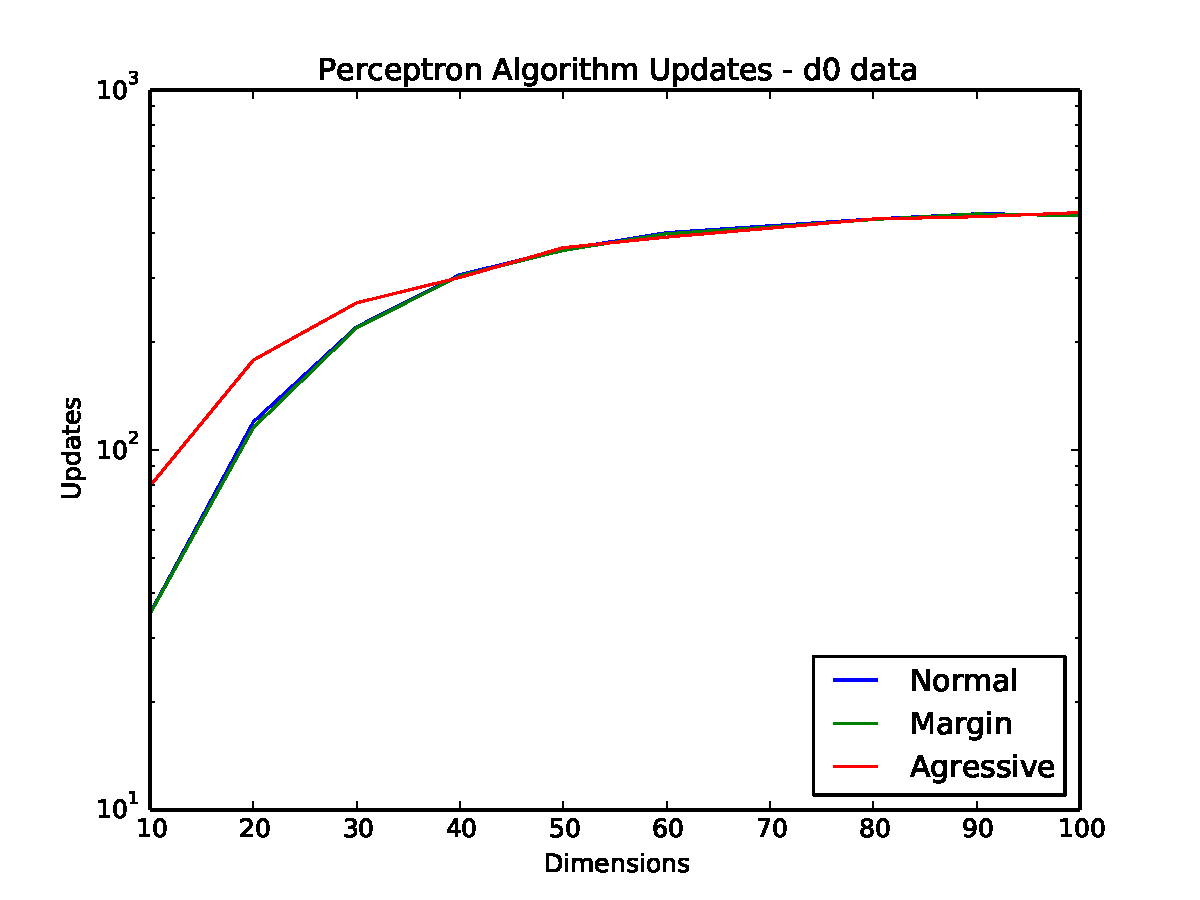
\includegraphics[width=\linewidth]{d0_updates.pdf}
  \captionof{figure}{Updates for {\tt data0}}
  \label{fig:updates_d0}
\end{minipage}%
\begin{minipage}{.5\textwidth}
  \centering
  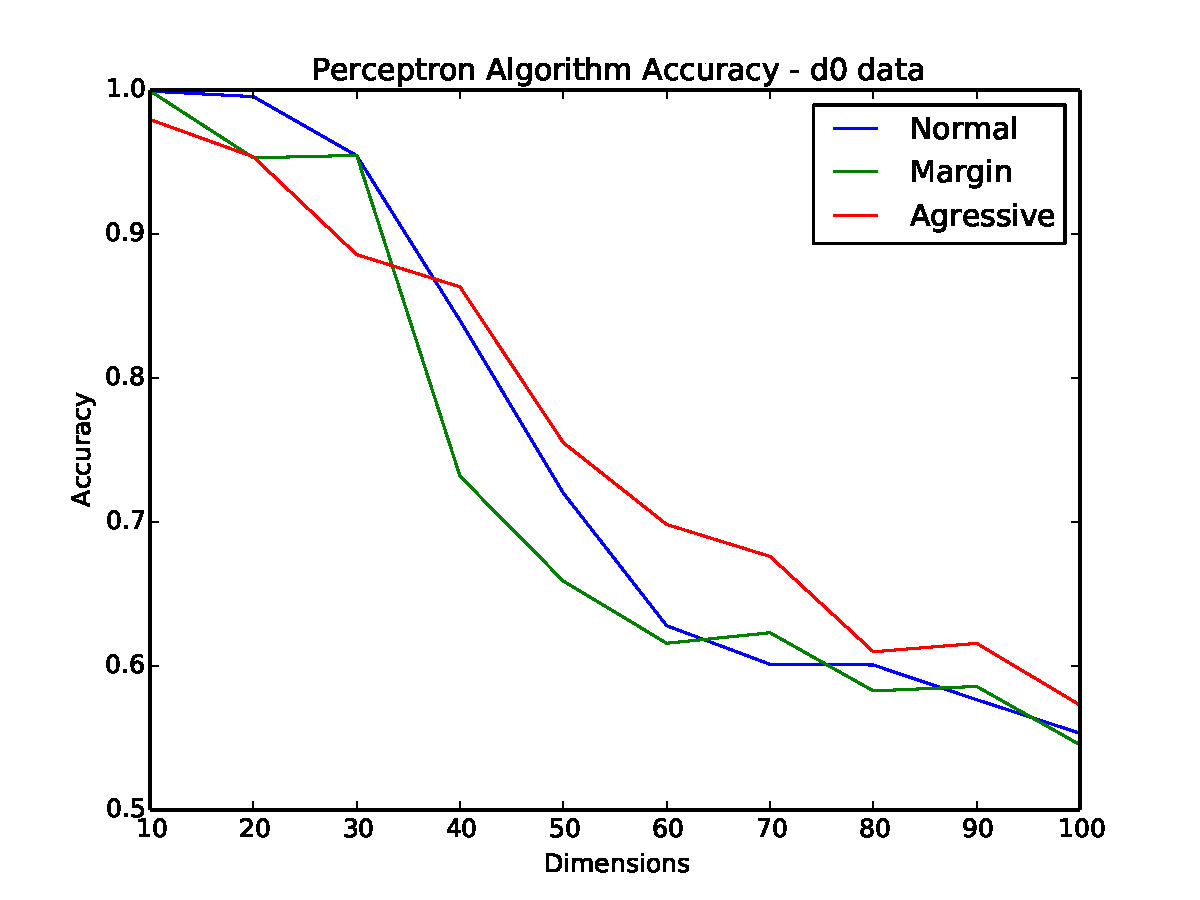
\includegraphics[width=\linewidth]{d0_accuracy.pdf}
  \captionof{figure}{Accuracy for {\tt data0}}
  \label{fig:accuracy_d0}
\end{minipage}
\end{figure}

Figure \ref{fig:updates_d0} shows the number of updates per algorithm for each of
the different Perceptron algorithms vs the dimensionality. This is only for the
dataset in \verb~data0~. As can be seen in the figures, the Margin Perceptron and
Normal Perceptron performed roughly the same, while the Agressive Perceptron required
more updates than either of the others, after which it performed roughly the same.

Seeing how this effects the accuracy in Figure \ref{fig:accuracy_d0}, up through 40
dimensions the Agressive Perceptron performs worse than the first two algorithms.
However, even though this is the case, the overall accuracy of the Agressive algorithm
drops off roughly linearly with the number of dimensions, while the other algorithms
drop off much quicker in accuracy for the dimensionality greater than 40.

\begin{figure}[H]
\centering
\begin{minipage}{.5\textwidth}
  \centering
  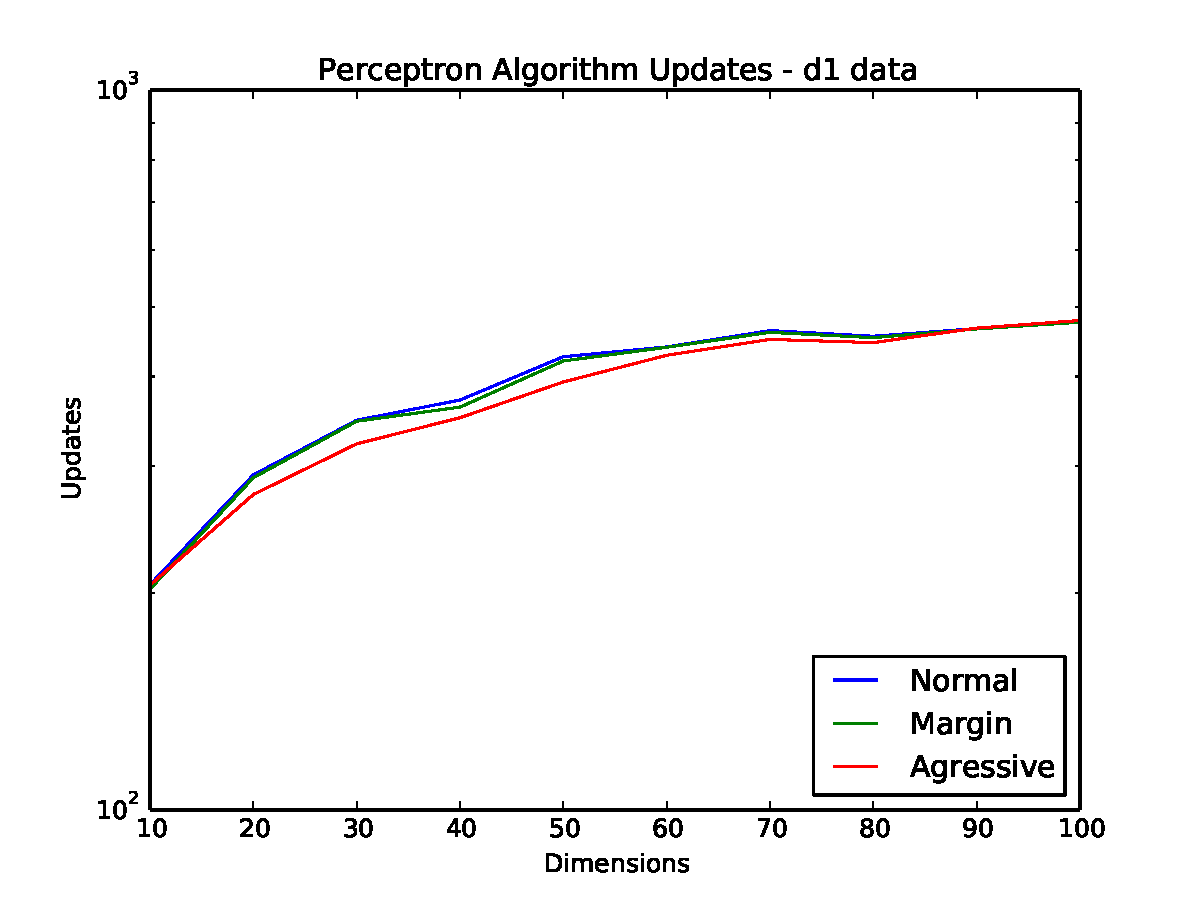
\includegraphics[width=\linewidth]{d1_updates.pdf}
  \captionof{figure}{Updates for {\tt data1}}
  \label{fig:updates_d1}
\end{minipage}%
\begin{minipage}{.5\textwidth}
  \centering
  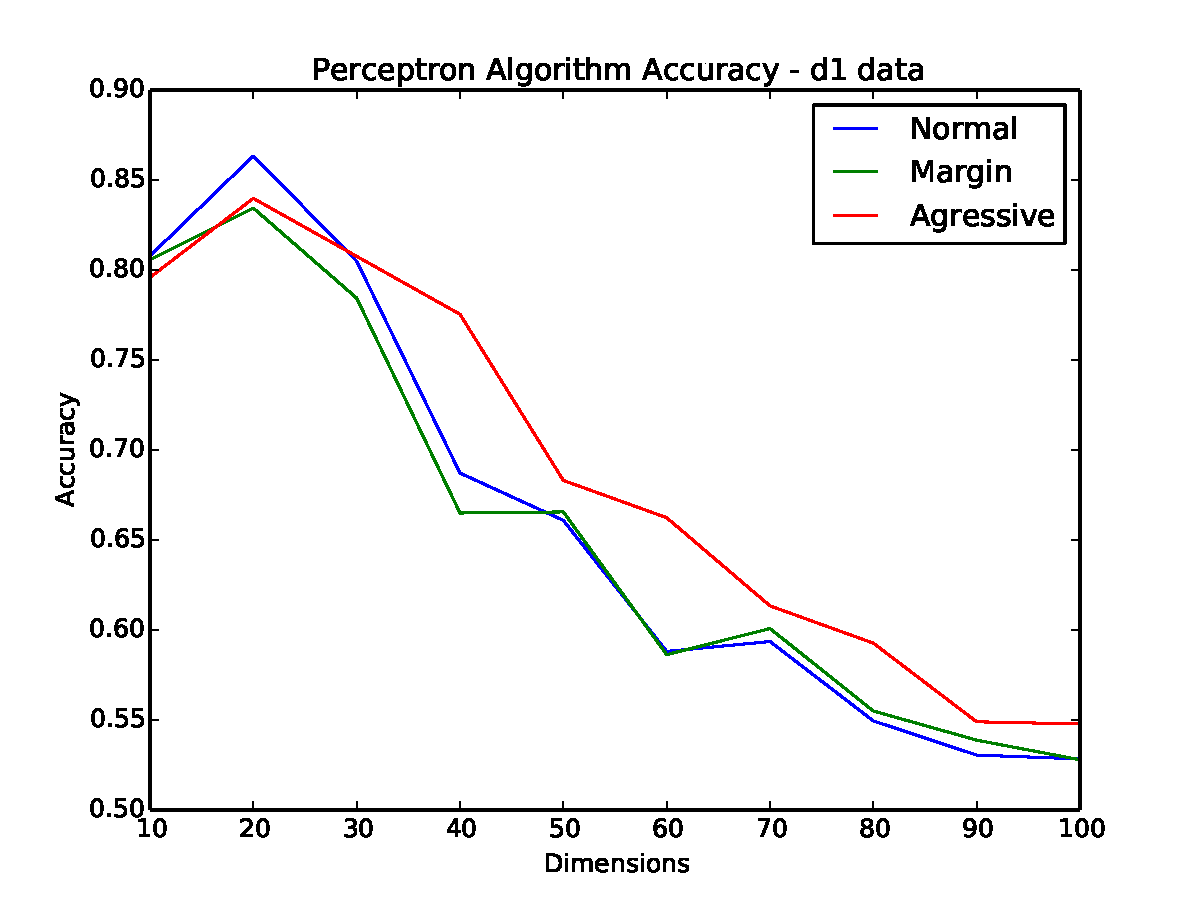
\includegraphics[width=\linewidth]{d1_accuracy.pdf}
  \captionof{figure}{Accuracy for {\tt data1}}
  \label{fig:accuracy_d1}
\end{minipage}
\end{figure}

Figure \ref{fig:updates_d1} shows the number of updates for each of the different
Perceptron algorithms vs dimensionality for \verb~data1~. The difference between
this set of data and the first set is that for the number of updates the Agressive
Perceptron algorithm seems to do better when looking at the number of updates.
The Margin Perceptron and Normal Perceptron perform relatively the same.

The results of this shows up in \ref{fig:accuracy_d1}. When compared to the accuracy
that is in Figure \ref{fig:accuracy_d0} from \verb~data0~, all of the algorithms
perform much less accurate than their counterparts in Figure \ref{fig:accuracy_d0}.
However, the drop in the amount of accuracy is much more for both the Margin Perceptron
and the Normal Perceptron Algorithms. In other words, the Agressive Perceptron algorithm
performed much better than the other two in this data set, which was not the case for
\verb~data0~.

Overall, out of the 3 different algorithms, the Agressive Perceptron algorithm
performs better for higher dimensional data when compared to either of the other two.
This is most likely because when updating the weight vector with $\eta$, you're dividing by the norm of $x$ which allows for it to be less susceptible to noise. On top of this, the Agressive
Perceptron also did better than both in \verb~data1~ than \verb~data0~ and did
not loose as much in accuracy. Again, this is most likely because of there being more noise in the second set of data and the agressive persceptron is less sensitive to this.
The Agressive Perceptron Algorithm seems to drop of linearly with respect to the dimensions
while the other two are more sensitive to the number of dimensions.


  \paragraph{Explanation of the update} We call this the aggressive
  update because the learning rate is derived from the following
  optimization problem:

  When we see that $y(\bw^T \bx) \leq \mu$, we try to find new values
  of $\bw$ such that $y(\bw^T \bx) = \mu$ using
  %
  \begin{eqnarray*}
    \min_{\bw_{new}} &     \frac{1}{2} {||\textbf{$\bw_{new}$} - \textbf{$\bw_{old}$}||}^2\\
    \mbox{such that} & y(\bw^T x) = \mu.
  \end{eqnarray*}
  %
  That is, the goal is to find the smallest change in the weights so
  that the current example is on the right side of the weight vector.

  By substituting (a) from above into this optimization problem, we
  will get a single variable optimization problem whose solution gives
  us the $\eta$ defined above. You can think of this algorithm as
  trying to tune the weight vector so that the current example is
  correctly classified right after the update.
\end{enumerate}


\subsection*{Submission Guidelines}

\begin{enumerate}
\item The report should detail your experiments. For each step,
  explain in no more than a paragraph or so how your implementation
  works.

\item {\em Your code should run on the CADE machines}. You should
  include a shell script, {\tt run.sh}, that will execute your code
  in the CADE environment. Your code should produce similar output
  to what you include in your report.

  You are responsible for ensuring that the grader can execute the
  code using only the included script. If you are using an
  esoteric programming language, you should make sure that its
  runtime is available on CADE.


\item Please do not hand in binary files! We will {\em not} grade
  binary submissions.

\end{enumerate}

%%% Local Variables:
%%% mode: latex
%%% TeX-master: "hw2"
%%% End:


\section{HAPPY HOLIDAYS Extra Credit}
\label{sec:logistic-regression}
\textbf{25pts} You've seen stochastic gradient decent applied to
logistic regression. Now we ask why this is a viable strategy for
optimizing this objective. Prove that SGD will find the optimal value
for this function. This can be done by demonstrating that the
objective is convex. There are many ways to prove this. One of the
most straightforward ways to show this is demonstrate that the Hessian
is positive-semidefninite.
\begin{enumerate}
\item ~[5 points] Find the Gradient of:
\[\sum_{i=1}^m \log\P{1+ \exp(-y_i\mathbf{w}^T\mathbf{x}_i)} + \frac{1}{\sigma^2}\mathbf{w}^T\mathbf{w}\]
\begin{itemize}
\item The gradient of any function is defined as
\begin{align}
\Grad{f(\mathbf{x})} &= \sum_{i=1}^{\mathcal{D}}\frac{\partial f(\mathbf{x})}{\partial x_{i}}\hat{e}_{i}\\
\intertext{where $\mathcal{D}$ is the dimensionality/number of dependent variables in $f(\mathbf{x})$ and $\hat{e}_{i}$ is the normal vector for that coordinate -- a value of 1 for all dimensions in cartesian space. This requires a derivative over $\mathbf{x}$ and $\mathbf{w}$ which is}
\Grad{f(\mathbf{x}_{i})} &= \sum_{i=1}^{\mathcal{D}}\frac{\partial f(\mathbf{x}_{i})}{\partial \mathbf{w}} + \frac{\partial f(\mathbf{x}_{i})}{\partial \mathbf{x}_{i}}\\
\intertext{We can rewrite our equation $f(\mathbf{x}_{i})$ to make it easier to differentiate}
f(\mathbf{x}_{i}) &= \sum_{i=1}^{n}\log\P{1+\exp(-y_{i}\mathbf{w}^{T}\mathbf{x}_{i})} + \frac{\left|\left| \mathbf{w}\right|\right|^{2}}{\sigma^{2}}\\
\intertext{where the derivative of a sum of a function is the sum of the derivative of that function, so the differentials can be brought inside the sum and the respected differentials can be taken and the partial derivative outside the braces denotes that segment representing that differential of $f(\mathbf{x}_{i})$}
\Grad{f(\mathbf{x}_{i})} &= \left\{ \sum_{i=1}^{n}\frac{-y_{i}\mathbf{x}_{i}}{\exp(y_{i}\mathbf{w}^{T}\mathbf{x}_{i})+1} + \frac{2\left|\left|\mathbf{w}\right|\right|}{\sigma^{2}}\right\}_{\frac{\partial f}{\partial \mathbf{w}}} + \left\{ \sum_{i=1}^{n}\frac{-y_{i}\mathbf{w}^{T}}{\exp(y_{i}\mathbf{w}^{T}\mathbf{x}_{i})+1} \right\}_{\frac{\partial f}{\partial \mathbf{x}}}
\end{align}
\end{itemize}
\item ~[5 points] Find the Hessian of (a).
\begin{itemize}
\item The Hessian Matrix is defined as
\begin{align}
\boldsymbol{\mathcal{H}}\left(f(\mathbf{x}_{i})\right) &= \left[ \begin{array}{l l}
\frac{\partial^{2}f}{\partial \mathbf{x}_{i}^{2}} & \frac{\partial^{2}f}{\partial \mathbf{x}_{i}\partial \mathbf{w}}\\
\frac{\partial^{2}f}{\partial \mathbf{w} \partial \mathbf{x}_{i}} & \frac{\partial^{2}f}{\partial \mathbf{w}^{2}}
\end{array} \right]\\
\frac{\partial^{2}f(\mathbf{x}_{i})}{\partial \mathbf{x}_{i}^{2}} &= \sum_{i=1}^{n} \frac{\left|\left|\mathbf{w}\right|\right|^{2}y_{i}^{2}e^{\varsigma_{i}}}{\left(e^{\varsigma_{i}}+1\right)^{2}}\\
\frac{\partial^{2}f(\mathbf{x}_{i})}{\partial \mathbf{x}_{i}\partial \mathbf{w}} &= \sum_{i=1}^{n}\frac{y_{i}\left[e^{\varsigma_{i}}\left(\varsigma_{i}-1\right)-1\right]}{\left(e^{\varsigma_{i}}+1\right)^{2}}\\
\frac{\partial^{2}f(\mathbf{x}_{i})}{\partial \mathbf{w} \partial \mathbf{x}_{i}} &= \frac{\partial^{2}f(\mathbf{x}_{i})}{\partial \mathbf{x}_{i}\partial \mathbf{w}} = \sum_{i=1}^{n}\frac{y_{i}\left[e^{\varsigma_{i}}\left(\varsigma_{i}-1\right)-1\right]}{\left(e^{\varsigma_{i}}+1\right)^{2}}\\
\frac{\partial^{2}f(\mathbf{x}_{i})}{\partial \mathbf{w}^{2}} &= \sum_{i=1}^{n}\frac{\left|\left|\mathbf{x}_{i}\right|\right|^{2}y_{i}^{2}e^{\varsigma_{i}}}{\left(e^{\varsigma_{i}}+1\right)^{2}}+\frac{2}{\sigma^{2}}
\intertext{where $\varsigma_{i} = \mathbf{w}^{T}\mathbf{x}_{i}y_{i}$}\nonumber
\end{align}
\end{itemize}
\item ~[10 points] prove that the Hessian is positive semidefinite.
\begin{itemize}
\item A matrix is {\em positive semidefinite} if and only if $\mathbf{b}^{T}\boldsymbol{\mathcal{H}}\mathbf{b}>\vec{0}\ \forall\ \mathbf{b}\neq\vec{0}$, where $\mathbf{b}$ is a vector. $\boldsymbol{\mathcal{H}}(f(\mathbf{x}_{i}))$ can be re-written as, by using Einstein Summation Notation
\begin{align}
\boldsymbol{\mathcal{H}} &= \left[ \begin{array}{l l}
\frac{\left|\left|\mathbf{w}\right|\right|^{2}y_{i}^{2}e^{\varsigma_{i}}}{\left(e^{\varsigma_{i}}+1\right)^{2}} & \frac{y_{i}\left[e^{\varsigma_{i}}\left(\varsigma_{i}-1\right)-1\right]}{\left(e^{\varsigma_{i}}+1\right)^{2}}\\
\frac{y_{i}\left[e^{\varsigma_{i}}\left(\varsigma_{i}-1\right)-1\right]}{\left(e^{\varsigma_{i}}+1\right)^{2}} & \frac{\left|\left|\mathbf{x}_{i}\right|\right|^{2}y_{i}^{2}e^{\varsigma_{i}}}{\left(e^{\varsigma_{i}}+1\right)^{2}}+\frac{2}{\sigma^{2}}
\end{array} \right]\\
\intertext{where $\varsigma_{i} = \mathbf{w}^{T}\mathbf{x}_{i}y_{i}$}\nonumber
\intertext{We only care about if it is going to be negative, so without loss of generality we can remove all the norms, squares, and denominators since they are {\em always} positive. We can also generalize our vector $\mathbf{b}$ as $\mathbf{b} = \left(\alpha_{1},\alpha_{2}\right)^{T}$, where $\alpha_{1}$ and $\alpha_{2}$ can be anything}
\boldsymbol{\mathcal{H}}^{\prime} &= \left[ \begin{array}{l l}
e^{\varsigma_{i}} & e^{\varsigma_{i}}(\varsigma_{i}-1)-1\\
e^{\varsigma_{i}}(\varsigma_{i}-1)-1 & e^{\varsigma_{i}}+\frac{2}{\sigma^{2}}
\end{array} \right]\\
\intertext{where $\mathbf{b}^{T}\boldsymbol{\mathcal{H}}^{\prime}\mathbf{b}$ can be generalized with the following result}
\mathbf{b}^{T} \left[\begin{array}{l l} x_{1} & x_{2}\\ x_{3} & x_{4}\end{array}\right]    \mathbf{b} &= x_{1}\alpha_{1}^{2} + x_{4}\alpha_{2}^{2} + \alpha_{1}\alpha_{2}(x_{2}+x_{3})\\
\intertext{when applied to $\boldsymbol{\mathcal{H}}^{\prime}$ results in}
\mathbf{b}^{T}\boldsymbol{\mathcal{H}}^{\prime}\mathbf{b} &= \alpha_{1}^{2}e^{\varsigma_{i}} + \alpha_{2}^{2}\left(e^{\varsigma_{i}}+\frac{2}{\sigma^{2}}\right) + 2\alpha_{1}\alpha_{2}\left(e^{\varsigma_{i}}(\varsigma_{i}-1)-1 \right)\\
\intertext{Where there's two instances that we need to prove. (1) If $\alpha_{1},\alpha_{2}>0$ then $\alpha_{1}\alpha_{2}(x_{2}+x_{3})>0$ and (2) if $\alpha_{1}>0$ and $\alpha_{2}<0$, then $\alpha_{1}^{2}x_{1}+\alpha_{2}^{2}x_{2}>\alpha_{1}\alpha_{2}(x_{2}+x_{3})$.}
\alpha_{1},\alpha_{2}>0 \Rightarrow \alpha_{1}\alpha_{2}(x_{2}+x_{3})>0\\
\alpha_{1}\alpha_{2}(x_{2}+x_{3}) &= 2\alpha_{1}\alpha_{2}\varsigma_{i}e^{\varsigma_{i}}-2e^{\varsigma_{i}}-2>0\\
&\underbrace{\varsigma_{i}e^{\varsigma_{i}}-e^{\varsigma_{i}}-1}_{>\ 0\text{ if }\varsigma_{i}e^{\varsigma_{i}}>e^{\varsigma_{i}}-1};\quad\varsigma_{i}\neq 0\\
&\Rightarrow \varsigma_{i}e^{\varsigma_{i}}>e^{\varsigma_{i}}-1\\
&\Rightarrow \varsigma_{i}>1-e^{-\varsigma_{i}}\qed
\intertext{where $\varsigma_{i}\geq 1\ \forall\ i$. Now for the alternative case where if $\alpha_{1}>0$ and $\alpha_{2}<0$, that $\alpha_{1}^{2}x_{1}+\alpha_{2}^{2}x_{2}>\alpha_{1}\alpha_{2}(x_{2}+x_{3})$}
\alpha_{1}^{2}e^{\varsigma_{i}}+\alpha_{2}^{2}\left(e^{\varsigma_{i}}+\frac{2}{\sigma^{2}}\right) &> \alpha_{1}\alpha_{2}\left[ e^{\varsigma_{i}}(\varsigma_{i}-1)-1 \right]\\
\left[ \alpha_{1}^{2} + \alpha_{2}^{2} + \frac{2}{\sigma^{2}e^{\varsigma_{i}}}\right] &> \left[ \alpha_{1}\alpha_{2}(\varsigma_{i}-1)-e^{-\varsigma_{i}} \right]\\
\intertext{if $\varsigma_{i}\gg 1$}
\underbrace{\alpha_{1}^{2}+\alpha_{2}^{2}}_{>\ 0} &> \underbrace{\alpha_{1}\alpha_{2}}_{<\ 0}\underbrace{\left(\varsigma_{i}-1 \right)}_{>\ 0}\qed
\intertext{for $\varsigma_{i}\geq 0$ (always)}
\underbrace{\alpha_{1}^{2}+\alpha_{2}^{2}}_{>\ 0}+\underbrace{e^{-\varsigma_{i}}}_{\geq\ 1}\underbrace{\left(\frac{2}{\sigma^{2}}+1\right)}_{>\ 0} &> \underbrace{\alpha_{1}\alpha_{2}}_{<\ 0}\underbrace{(\varsigma_{i}-1)}_{>\ 0}\qed
\end{align}
\end{itemize}
\item ~[5 points] Why does this prove that we are GUARANTEED to have within $\epsilon>0$ of the right answer?
\begin{itemize}
\item Because the Hessian Matrix of the function is positive-semidefinite, the given function is convex. On top of which, since we are maximizing the function, we are required to step with the gradient and stop when the slope is less than some tolerance $(\epsilon)$. The gradient gives the slope/direction of the greatest change and we ``walk'' in teh direction which makes the gradient zero. We are guarenteed that one exists since the Hessian is positive-semidefinite.
\end{itemize}
\end{enumerate}

%%% Local Variables:
%%% mode: latex
%%% TeX-master: "hw5"
%%% End:


\end{document}
%%% Local Variables:
%%% mode: latex
%%% TeX-master: t
%%% End:
